\documentclass{ximera}

%\usepackage{todonotes}

\newcommand{\todo}{}

\usepackage{esint} % for \oiint
\ifxake%%https://math.meta.stackexchange.com/questions/9973/how-do-you-render-a-closed-surface-double-integral
\renewcommand{\oiint}{{\large\bigcirc}\kern-1.56em\iint}
\fi


\graphicspath{
  {./}
  {ximeraTutorial/}
  {basicPhilosophy/}
  {functionsOfSeveralVariables/}
  {normalVectors/}
  {lagrangeMultipliers/}
  {vectorFields/}
  {greensTheorem/}
  {shapeOfThingsToCome/}
  {dotProducts/}
  {partialDerivativesAndTheGradientVector/}
  {../productAndQuotientRules/exercises/}
  {../normalVectors/exercisesParametricPlots/}
  {../continuityOfFunctionsOfSeveralVariables/exercises/}
  {../partialDerivativesAndTheGradientVector/exercises/}
  {../directionalDerivativeAndChainRule/exercises/}
  {../commonCoordinates/exercisesCylindricalCoordinates/}
  {../commonCoordinates/exercisesSphericalCoordinates/}
  {../greensTheorem/exercisesCurlAndLineIntegrals/}
  {../greensTheorem/exercisesDivergenceAndLineIntegrals/}
  {../shapeOfThingsToCome/exercisesDivergenceTheorem/}
  {../greensTheorem/}
  {../shapeOfThingsToCome/}
  {../separableDifferentialEquations/exercises/}
  {vectorFields/}
}

\newcommand{\mooculus}{\textsf{\textbf{MOOC}\textnormal{\textsf{ULUS}}}}

\usepackage{tkz-euclide}
\usepackage{tikz}
\usepackage{tikz-cd}
\usetikzlibrary{arrows}
\tikzset{>=stealth,commutative diagrams/.cd,
  arrow style=tikz,diagrams={>=stealth}} %% cool arrow head
\tikzset{shorten <>/.style={ shorten >=#1, shorten <=#1 } } %% allows shorter vectors

\usetikzlibrary{backgrounds} %% for boxes around graphs
\usetikzlibrary{shapes,positioning}  %% Clouds and stars
\usetikzlibrary{matrix} %% for matrix
\usepgfplotslibrary{polar} %% for polar plots
\usepgfplotslibrary{fillbetween} %% to shade area between curves in TikZ
%\usetkzobj{all}
\usepackage[makeroom]{cancel} %% for strike outs
%\usepackage{mathtools} %% for pretty underbrace % Breaks Ximera
%\usepackage{multicol}
\usepackage{pgffor} %% required for integral for loops



%% http://tex.stackexchange.com/questions/66490/drawing-a-tikz-arc-specifying-the-center
%% Draws beach ball
\tikzset{pics/carc/.style args={#1:#2:#3}{code={\draw[pic actions] (#1:#3) arc(#1:#2:#3);}}}



\usepackage{array}
\setlength{\extrarowheight}{+.1cm}
\newdimen\digitwidth
\settowidth\digitwidth{9}
\def\divrule#1#2{
\noalign{\moveright#1\digitwidth
\vbox{\hrule width#2\digitwidth}}}




% \newcommand{\RR}{\mathbb R}
% \newcommand{\R}{\mathbb R}
% \newcommand{\N}{\mathbb N}
% \newcommand{\Z}{\mathbb Z}

\newcommand{\sagemath}{\textsf{SageMath}}


%\renewcommand{\d}{\,d\!}
%\renewcommand{\d}{\mathop{}\!d}
%\newcommand{\dd}[2][]{\frac{\d #1}{\d #2}}
%\newcommand{\pp}[2][]{\frac{\partial #1}{\partial #2}}
% \renewcommand{\l}{\ell}
%\newcommand{\ddx}{\frac{d}{\d x}}

% \newcommand{\zeroOverZero}{\ensuremath{\boldsymbol{\tfrac{0}{0}}}}
%\newcommand{\inftyOverInfty}{\ensuremath{\boldsymbol{\tfrac{\infty}{\infty}}}}
%\newcommand{\zeroOverInfty}{\ensuremath{\boldsymbol{\tfrac{0}{\infty}}}}
%\newcommand{\zeroTimesInfty}{\ensuremath{\small\boldsymbol{0\cdot \infty}}}
%\newcommand{\inftyMinusInfty}{\ensuremath{\small\boldsymbol{\infty - \infty}}}
%\newcommand{\oneToInfty}{\ensuremath{\boldsymbol{1^\infty}}}
%\newcommand{\zeroToZero}{\ensuremath{\boldsymbol{0^0}}}
%\newcommand{\inftyToZero}{\ensuremath{\boldsymbol{\infty^0}}}



% \newcommand{\numOverZero}{\ensuremath{\boldsymbol{\tfrac{\#}{0}}}}
% \newcommand{\dfn}{\textbf}
% \newcommand{\unit}{\,\mathrm}
% \newcommand{\unit}{\mathop{}\!\mathrm}
% \newcommand{\eval}[1]{\bigg[ #1 \bigg]}
% \newcommand{\seq}[1]{\left( #1 \right)}
% \renewcommand{\epsilon}{\varepsilon}
% \renewcommand{\phi}{\varphi}


% \renewcommand{\iff}{\Leftrightarrow}

% \DeclareMathOperator{\arccot}{arccot}
% \DeclareMathOperator{\arcsec}{arcsec}
% \DeclareMathOperator{\arccsc}{arccsc}
% \DeclareMathOperator{\si}{Si}
% \DeclareMathOperator{\scal}{scal}
% \DeclareMathOperator{\sign}{sign}


%% \newcommand{\tightoverset}[2]{% for arrow vec
%%   \mathop{#2}\limits^{\vbox to -.5ex{\kern-0.75ex\hbox{$#1$}\vss}}}
% \newcommand{\arrowvec}[1]{{\overset{\rightharpoonup}{#1}}}
% \renewcommand{\vec}[1]{\arrowvec{\mathbf{#1}}}
% \renewcommand{\vec}[1]{{\overset{\boldsymbol{\rightharpoonup}}{\mathbf{#1}}}}

% \newcommand{\point}[1]{\left(#1\right)} %this allows \vector{ to be changed to \vector{ with a quick find and replace
% \newcommand{\pt}[1]{\mathbf{#1}} %this allows \vec{ to be changed to \vec{ with a quick find and replace
% \newcommand{\Lim}[2]{\lim_{\point{#1} \to \point{#2}}} %Bart, I changed this to point since I want to use it.  It runs through both of the exercise and exerciseE files in limits section, which is why it was in each document to start with.

% \DeclareMathOperator{\proj}{\mathbf{proj}}
% \newcommand{\veci}{{\boldsymbol{\hat{\imath}}}}
% \newcommand{\vecj}{{\boldsymbol{\hat{\jmath}}}}
% \newcommand{\veck}{{\boldsymbol{\hat{k}}}}
% \newcommand{\vecl}{\vec{\boldsymbol{\l}}}
% \newcommand{\uvec}[1]{\mathbf{\hat{#1}}}
% \newcommand{\utan}{\mathbf{\hat{t}}}
% \newcommand{\unormal}{\mathbf{\hat{n}}}
% \newcommand{\ubinormal}{\mathbf{\hat{b}}}

% \newcommand{\dotp}{\bullet}
% \newcommand{\cross}{\boldsymbol\times}
% \newcommand{\grad}{\boldsymbol\nabla}
% \newcommand{\divergence}{\grad\dotp}
% \newcommand{\curl}{\grad\cross}
%\DeclareMathOperator{\divergence}{divergence}
%\DeclareMathOperator{\curl}[1]{\grad\cross #1}
% \newcommand{\lto}{\mathop{\longrightarrow\,}\limits}

% \renewcommand{\bar}{\overline}

\colorlet{textColor}{black}
\colorlet{background}{white}
\colorlet{penColor}{blue!50!black} % Color of a curve in a plot
\colorlet{penColor2}{red!50!black}% Color of a curve in a plot
\colorlet{penColor3}{red!50!blue} % Color of a curve in a plot
\colorlet{penColor4}{green!50!black} % Color of a curve in a plot
\colorlet{penColor5}{orange!80!black} % Color of a curve in a plot
\colorlet{penColor6}{yellow!70!black} % Color of a curve in a plot
\colorlet{fill1}{penColor!20} % Color of fill in a plot
\colorlet{fill2}{penColor2!20} % Color of fill in a plot
\colorlet{fillp}{fill1} % Color of positive area
\colorlet{filln}{penColor2!20} % Color of negative area
\colorlet{fill3}{penColor3!20} % Fill
\colorlet{fill4}{penColor4!20} % Fill
\colorlet{fill5}{penColor5!20} % Fill
\colorlet{gridColor}{gray!50} % Color of grid in a plot

\newcommand{\surfaceColor}{violet}
\newcommand{\surfaceColorTwo}{redyellow}
\newcommand{\sliceColor}{greenyellow}




\pgfmathdeclarefunction{gauss}{2}{% gives gaussian
  \pgfmathparse{1/(#2*sqrt(2*pi))*exp(-((x-#1)^2)/(2*#2^2))}%
}


%%%%%%%%%%%%%
%% Vectors
%%%%%%%%%%%%%

%% Simple horiz vectors
\renewcommand{\vector}[1]{\left\langle #1\right\rangle}


%% %% Complex Horiz Vectors with angle brackets
%% \makeatletter
%% \renewcommand{\vector}[2][ , ]{\left\langle%
%%   \def\nextitem{\def\nextitem{#1}}%
%%   \@for \el:=#2\do{\nextitem\el}\right\rangle%
%% }
%% \makeatother

%% %% Vertical Vectors
%% \def\vector#1{\begin{bmatrix}\vecListA#1,,\end{bmatrix}}
%% \def\vecListA#1,{\if,#1,\else #1\cr \expandafter \vecListA \fi}

%%%%%%%%%%%%%
%% End of vectors
%%%%%%%%%%%%%

%\newcommand{\fullwidth}{}
%\newcommand{\normalwidth}{}



%% makes a snazzy t-chart for evaluating functions
%\newenvironment{tchart}{\rowcolors{2}{}{background!90!textColor}\array}{\endarray}

%%This is to help with formatting on future title pages.
\newenvironment{sectionOutcomes}{}{}



%% Flowchart stuff
%\tikzstyle{startstop} = [rectangle, rounded corners, minimum width=3cm, minimum height=1cm,text centered, draw=black]
%\tikzstyle{question} = [rectangle, minimum width=3cm, minimum height=1cm, text centered, draw=black]
%\tikzstyle{decision} = [trapezium, trapezium left angle=70, trapezium right angle=110, minimum width=3cm, minimum height=1cm, text centered, draw=black]
%\tikzstyle{question} = [rectangle, rounded corners, minimum width=3cm, minimum height=1cm,text centered, draw=black]
%\tikzstyle{process} = [rectangle, minimum width=3cm, minimum height=1cm, text centered, draw=black]
%\tikzstyle{decision} = [trapezium, trapezium left angle=70, trapezium right angle=110, minimum width=3cm, minimum height=1cm, text centered, draw=black]


\title{Periodic Functions}

\begin{document}

\begin{abstract}
repeating
\end{abstract}
\maketitle



In addition to gluing together pieces from several functions, we also have functions which just repeat one part over and over and over. They glue the same function next to itself over and over and over.  These functions are said to be \textbf{periodic}.









\begin{example}  \textit{Sawtooth Functions} \\


Let's begin with a function whose graph looks like an iscoceles triangle.


Graph of $y = Tooth(t)$.
\begin{image}
\begin{tikzpicture}
	\begin{axis}[
            domain=-10:10, ymax=2, xmax=10, ymin=-2, xmin=-10,
            axis lines =center, xlabel=$t$, ylabel=$y$,
            ytick={-2,-1,1,2},
            xtick={-10,-8,-6,-4,-2,2,4,6,8,10},
            ticklabel style={font=\scriptsize},
            every axis y label/.style={at=(current axis.above origin),anchor=south},
            every axis x label/.style={at=(current axis.right of origin),anchor=west},
            axis on top
          ]
          

	\addplot [draw=penColor,very thick,smooth,domain=(0:1)] {x};
	\addplot [draw=penColor,very thick,smooth,domain=(1:2)] {-x+2};



    \end{axis}
\end{tikzpicture}
\end{image}





The tooth here is $1$ unit high and $2$ units wide and this Sawtooth function below just repeats this tooth over and over and over.



Graph of $y = SawTooth(t)$.
\begin{image}
\begin{tikzpicture}
	\begin{axis}[
            domain=-10:10, ymax=2, xmax=10, ymin=-2, xmin=-10,
            axis lines =center, xlabel=$t$, ylabel=$y$,
            ytick={-2,-1,1,2},
            xtick={-10,-8,-6,-4,-2,2,4,6,8,10},
            ticklabel style={font=\scriptsize},
            every axis y label/.style={at=(current axis.above origin),anchor=south},
            every axis x label/.style={at=(current axis.right of origin),anchor=west},
            axis on top
          ]
          
	\addplot [draw=penColor,very thick,smooth,domain=(-2:-1)] {x+2};
	\addplot [draw=penColor,very thick,smooth,domain=(-1:0)] {-x};

	\addplot [draw=penColor,very thick,smooth,domain=(0:1)] {x};
	\addplot [draw=penColor,very thick,smooth,domain=(1:2)] {-x+2};

	\addplot [draw=penColor,very thick,smooth,domain=(2:3)] {x-2};
	\addplot [draw=penColor,very thick,smooth,domain=(3:4)] {-x+4};



	\addplot[color=penColor,only marks,mark=*] coordinates{(-3,0.5)}; 
	\addplot[color=penColor,only marks,mark=*] coordinates{(-4,0.5)}; 
	\addplot[color=penColor,only marks,mark=*] coordinates{(-5,0.5)}; 

	\addplot[color=penColor,only marks,mark=*] coordinates{(5,0.5)}; 
	\addplot[color=penColor,only marks,mark=*] coordinates{(6,0.5)}; 
	\addplot[color=penColor,only marks,mark=*] coordinates{(7,0.5)}; 




    \end{axis}
\end{tikzpicture}
\end{image}



\begin{question}
  \begin{itemize}
    \item $SawTooth(0) = \answer{0}$
    \item $SawTooth(1) = \answer{1}$
    \item $SawTooth(2) = \answer{0}$
    \item $SawTooth(57) = \answer{1}$
    \item $SawTooth(102) = \answer{0}$
  \end{itemize}
\end{question}

\end{example}



Different sawtooth functions are made by varying the height and width of the tooth.  The single tooth that was repeated is called the \textbf{wave} of the function.  The width of the wave is called the \textbf{period}. And, the height of the wave is called the \textbf{amplitude}.




Sawtooth functions are piecewise defined functions but there is really one piece that just repeats.  We would like to express this idea in a formula. We define a formula for the initial piece and then state the period.




\[
SawTooth(x) = 
\begin{cases}
  x &\text{on $[0,1)$,} \\
  -x+2 &\text{on $[1,2)$} \\ 
  SawTooth(x) = SawTooth(x+2) & \text{otherwise}
\end{cases}
\]


$SawTooth(x) = SawTooth(x+2)$ tells us to keep jumping by $2$ until you get to a known value.


\begin{example}


Evaluate  $SawTooth(9)$. \\

Using the equation $SawTooth(x) = SawTooth(x+2)$ several times, we get 


\[
SawTooth(9) = SawTooth(7) = SawTooth(5) = SawTooth(3) = SawTooth(1) = -(1) + 2 = 1
\]


\begin{question}

Evaluate.  $SawTooth(-2) = \answer{0}$ \\

Evaluate.  $SawTooth\left( \frac{5}{2} \right) = \answer{\frac{1}{2}}$ \\

Evaluate.  $SawTooth(401) = \answer{1}$

\end{question}


\end{example}








This function gets its name because it looks like moving up and down on the teeth on a saw. Other periodic functions come from similarly moving on different objects. 




You can make a periodic function out of any piece of any function, just use that piece as the wave. But we have two very special basic periodic functions in our set of Elementary Functions.



Travelling around the unit circle produces two important periodic functions.














\subsection*{The Unit Circle}


The unit circle is the circle of radius $1$ centered at the origin in the Cartesian plane. A point on the unit circle has two coordinates.  

\begin{itemize}
\item The first coordinate gives the horizontal position of the point. 
\item The second coordinate gives the vertical position of the point.  
\end{itemize}

Both of these depend on an angle measurement, $\theta$. $\theta$ is the angle made between the positive horizontal axis and a radius formed by drawing a line from the origin (center of the circle) the point on the unit circle.


\begin{example} \textit{Sine} and \textit{Cosine}  \\

\begin{image}
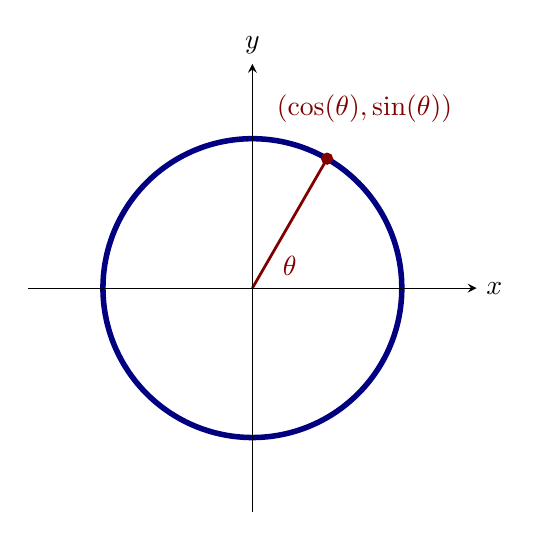
\begin{tikzpicture} 
  \begin{axis}[
            domain=-1.5:1.5, ymax=1.5, xmax=1.5, ymin=-1.5, xmin=-1.5,
            axis lines =center, unit vector ratio*=1 1 1, xlabel=$x$, ylabel=$y$,
            ytick={-10,-8,-6,-4,-2,2,4,6,8,10},
            xtick={-10,-8,-6,-4,-2,2,4,6,8,10},
            ticklabel style={font=\scriptsize},
            every axis y label/.style={at=(current axis.above origin),anchor=south},
            every axis x label/.style={at=(current axis.right of origin),anchor=west},
            axis on top
          ]
          
          	\addplot [line width=2, penColor, smooth,samples=100,domain=(0:6.3)] ({cos(deg(x))},{sin(deg(x)});


        	\addplot [color=penColor2,only marks,mark=*] coordinates{(0.5,0.866)};


        	%\draw[decoration={brace,raise=.2cm,mirror},decorate,thin] (axis cs:0.75,0)--(axis cs:0.75,0.866);
        	%\draw[decoration={brace,raise=.2cm},decorate,thin] (axis cs:0,0.95)--(axis cs:0.75,0.95);
        	%\node[anchor=east] at (axis cs:1.85,3) {$d$};
        	%\node[anchor=east] at (axis cs:4.6,1) {$f(d)$};
                     
        	\node at (axis cs:0.75,1.2) [penColor2] {$(\cos(\theta),\sin(\theta))$};


          \addplot [line width=1, penColor2, smooth,samples=100,domain=(0:0.5)] ({x},{1.7320*x});
          \node at (axis cs:0.25,0.15) [penColor2] {$\theta$};


          %\addplot [color=penColor,only marks,mark=*] coordinates{(-4,-1) (0,1) (1,-6.5) (7,-3.5)};

          %\addplot [line width=1, penColor2, smooth,samples=100,domain=(-4:0)] ({x},{0});
          %\addplot [line width=1, penColor2, smooth,samples=100,domain=(1:7)] ({x},{0});
           

  \end{axis}
\end{tikzpicture}
\end{image}



As the angle changes, the corresponding point on the unit circle changes position and thus its coordinates change.  In other words, given an angle, there is exactly one corresponding point in the unit circle at that angle.  

\begin{itemize}
\item Given an angle there is exactly one corresponding horizontal coordinate.
\item Given an angle there is exactly one corresponding vertical coordinate. 
\end{itemize}


The horizontal and vertical coordinates of points on the unit circle are functions of the angle.  These two functions are called \textbf{cosine} and \textbf{sine} - abbreviated as \textbf{cos} and \textbf{sin}.

Each point on the unit circle has coordinates described as 

\[  (\cos(\theta), \sin(\theta))  \] 

As the angle turns around the unit circle, these coordinates repeat. Sine and cosine are periodic functions.

\end{example}




\begin{remark}  Etymology


Where do the trigonometric names come from?  \link{https://mathisonian.github.io/trig/etymology/}

\end{remark}











\subsection*{Angle Measurement}

The domain of \textit{sine} and \textit{cosine} are real numbers interpreted as angle measurements measured couterclockwise from the positive horizontal axis.  We have two units for measuring these angles.


\begin{itemize}
\item \textbf{degrees:}  A full circle is divided into $360$ degrees.
\item \textbf{radians:}  A full circle is divided into $2\pi$ radians.
\end{itemize}


\begin{question} Pieces of a Circle
	\begin{itemize}
		\item A half-circle rotation is $\answer{180}$ degrees.
		\item A quarter-circle rotation is $\answer{90}$ degrees.
		\item A eighth-circle rotation is $\answer{45}$ degrees.
		\item A half-circle rotation s $\answer{\pi}$ radians.
		\item A quarter-circle rotation is $\answer{\frac{\pi}{2}}$ radians.
		\item A eighth-circle rotation is $\answer{\frac{\pi}{4}}$ radians.

	\end{itemize}
\end{question}


\textbf{Shorthand:}  Degrees has a little superscript circle as a shorthand abbreviations, like $90^\circ$.  Radians doesn't have a shorthand abbreviation.  Therefore, if you see an angle measurement with no units, then the units are radians. 

\begin{idea} \textbf{\textcolor{green!50!black}{Cosine}}
\begin{itemize}
\item With Degrees: \\
As the angle, $\theta$, rotates counter-clockwise from $0^\circ$, the value of cosine start at $1$, decreases to $0$ at $90^\circ$, keeps decreasing to $-1$ at $180^\circ$, increases to $0$ at $270^\circ$, keeps increasing to $1$ at $360^\circ$.  These values continue to repeat with a period of $360^\circ$.

\item With Radians: \\
As the angle, $\theta$, rotates counter-clockwise from $0^\circ$, the values of cosine start at $1$, decrease to $0$ at $\frac{\pi}{2}$, keeps decreasing to $-1$ at $\pi$, increases to $0$ at $\frac{3\pi}{2}$, keeps increasing to $1$ at $32\pi$.  These values continue to repeat with a period of $2\pi$.
\end{itemize}
\end{idea}



\begin{idea} \textbf{\textcolor{green!50!black}{Sine}}
\begin{itemize}
\item With Degrees: \\
As the angle, $\theta$, rotates counter-clockwise the value of sine start at $0$, increases to $1$ at $90^\circ$, decreases to $0$ at $180^\circ$, keeps decreasing to $-1$ at $270^\circ$, increases to $0$ at $360^\circ$.  These values continue to repeat with a period of $360^\circ$.

\item With Radians: \\
As the angle, $\theta$, rotates counter-clockwise the value of sine start at $0$, increases to $1$ at $\frac{\pi}{2}$, decreases to $0$ at $\pi$, keeps decreasing to $-1$ at $\frac{3\pi}{2}$, increases to $0$ at $2\pi$.  These values continue to repeat with a period of $2\pi$.
\end{itemize}
\end{idea}



Angles are measured counterclockwise from the positive horizontal axis.  It is like a circular number line.  Rotating counterclockwise is the positive direction.  Rotating clockwise is the negative direction.  After you rotate a full circle (positively or negatively), the values just keep repeating.



\begin{onlineOnly}

\begin{center}
\desmos{g0wxuza2rb}{800}{400}
\end{center}

\end{onlineOnly}




\begin{warning}
It turns out that there are many connections between sine and cosine. Many. One of these connections concerns rate of change, which is a very important thread in this course.  The easiest way to describe these connections is with radians. Hence, Calculus only uses radians. Therefore, we will attempt to speak in radians as much as possible.
\end{warning}



Sine and Cosine are periodic functions with periods of $2\pi$. Therefore, we only need examine the interval $[0, 2\pi)$ and then repeat our findings every $2\pi$. \\


We call the interval $[0, 2\pi)$, the \textbf{principle interval} for sine and cosine. \\

From the graphs we can see that Sine and Cosine have maximum and minimum values.



\begin{explanation}
\begin{itemize}

  \item The sine function has a maximum value of $\answer{1}$.  Inside the interval $[0, 2\pi)$, this maximum value of sine occurs at $\answer{\frac{\pi}{2}}$.

  \item The sine function has a minimum value of $\answer{-1}$.  Inside the interval $[0, 2\pi)$, this minimum value of since occurs at $\answer{\frac{3\pi}{2}}$.

  \item The sine function has two zeros inside the interval $[0, 2\pi)$. One of these zeros is $0$.  The other zero is $\answer{\pi}$.


\end{itemize}





\begin{itemize}
  
  \item The cosine function has a maximum value of $\answer{1}$.  Inside the interval $[0, 2\pi)$, this maximum value of cosine occurs at $\answer{0}$.

  \item The cosine function has a minimum value of $\answer{-1}$.  Inside the interval $[0, 2\pi)$, this minimum value of cosine occurs at $\answer{\pi}$.

  \item The cosine function has two zeros inside the interval $[0, 2\pi)$. One of these zeros is $\frac{\pi}{2}$.  The other zero is $\answer{\frac{3\pi}{2}}$.


\end{itemize}

\end{explanation}













\begin{onlineOnly}
\begin{center}
\textbf{\textcolor{green!50!black}{ooooo-=-=-=-ooOoo-=-=-=-ooooo}} \\

more examples can be found by following this link\\ \link[More Examples of Piecewise-Defined Functions]{https://ximera.osu.edu/csccmathematics/precalculus/precalculus/piecewise/examples/exampleList}

\end{center}
\end{onlineOnly}




\end{document}
